This section is new in this report. It explains where the gain of the final model comes from, using the conditional coverage of the intervals, a decomposition of the interval score, and a comparison with every alternative interval we could build (scripts \texttt{fr\_condcov.py} and \texttt{fr\_bootstrap.py}).

\begin{figure}[H]
  \centering
  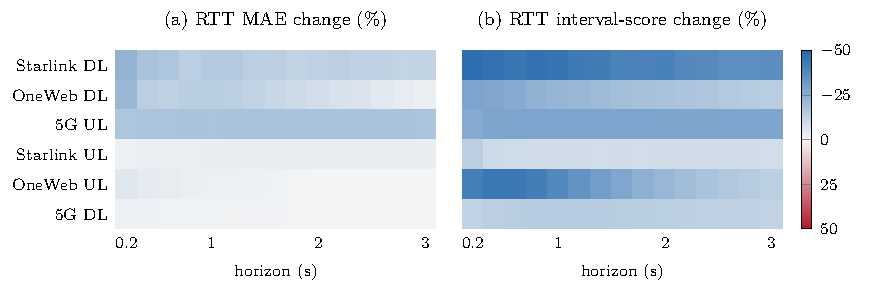
\includegraphics[width=0.9\linewidth]{figs_pdf/fr_heat.pdf}
  \caption{Change (\%) of the RTT MAE and of the calibrated 95\% interval score of DS2S-E against S2S-E per link and horizon step. Blue: DS2S-E is better.}
  \label{fig:heat}
\end{figure}

\subsection{The Gain Is in the Interval, at Every Horizon}
Fig.~\ref{fig:heat} shows the change of the RTT MAE and of the interval score of the final ensemble against the previous one for every link and horizon step. The interval score improves in every cell. The gain is largest at short horizons on the satellite links and flat on 5G. The MAE improves in every cell as well, but by much less on Starlink UL, OneWeb UL, and 5G DL. Almost all of the MAE gain comes from reporting the median instead of the mean. On the five links other than Starlink DL, the mean of DS2S-E changes the MAE by \MeanMAELo\% to $+$\MeanMAEHi\%, against \MedMAELo\% to \MedMAEHi\% for its median. Under right-skewed errors the median is closer to a typical outcome. Starlink DL is the one link where the mean also improves (\MeanMAESLDL\%), because its sawtooth is partly predictable.

\subsection{Conditional Coverage}
Fig.~\ref{fig:condcov} breaks the coverage down by the volatility of the input window (deciles of the input RTT SD, edges from the calibration sessions) and by the horizon. The constant interval of S2S-E is blue in the calm deciles and red in the volatile ones: it over-covers quiet windows and under-covers volatile ones. It covers the calmest tenth of the windows at \CovConstSLDLdOne{} and the most volatile tenth at \CovConstSLDLdTen{} on Starlink DL, and at \CovConstQULdOne{} and \CovConstQULdTen{} on 5G UL. Scaling the interval in proportion to the input SD with a small floor reverses the error (bottom row), because the future error grows much more slowly than the input SD (OneWeb DL calmest tenth: \CovNormOWDLdOne). The DS2S-E interval is close to white on Starlink DL and 5G UL. Its largest decile deviation from 0.95 (coverage gap) is \GapDSSLDL{} on Starlink DL, \GapDSQDL{} on 5G DL, and \GapDSQUL{} on 5G UL, against \GapConstSLDL{}, \GapConstQDL{}, and \GapConstQUL{} for the constant interval. The reduction is significant (paired session bootstrap) on these three links and on Starlink UL. Table~\ref{tab:condcovall} gives the gap and the interval score for every interval on every link.

\begin{figure}[H]
  \centering
  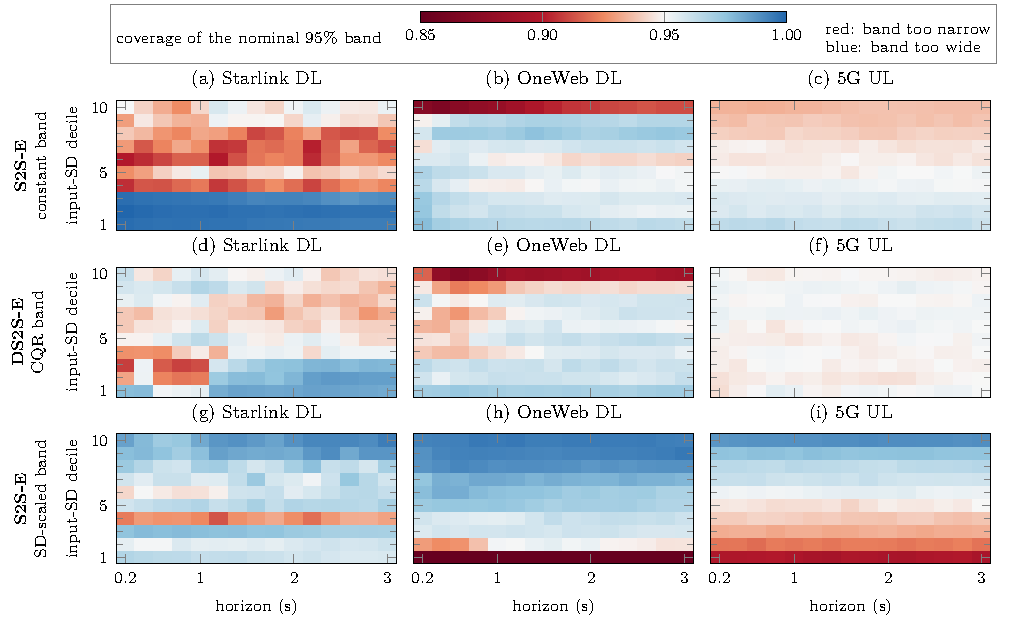
\includegraphics[width=\linewidth]{figs_pdf/fr_condcov.pdf}
  \caption{Conditional coverage of the calibrated 95\% RTT intervals on the test sessions. A cell is the coverage among the windows whose input SD lies in that decile at that horizon step. White: nominal 0.95. Blue: the interval is wider than needed. Red: it is too narrow. Values below 0.85 share the darkest red. Bottom row: interval scaled by the input SD with a small floor.}
  \label{fig:condcov}
\end{figure}

\begin{figure}[H]
  \centering
  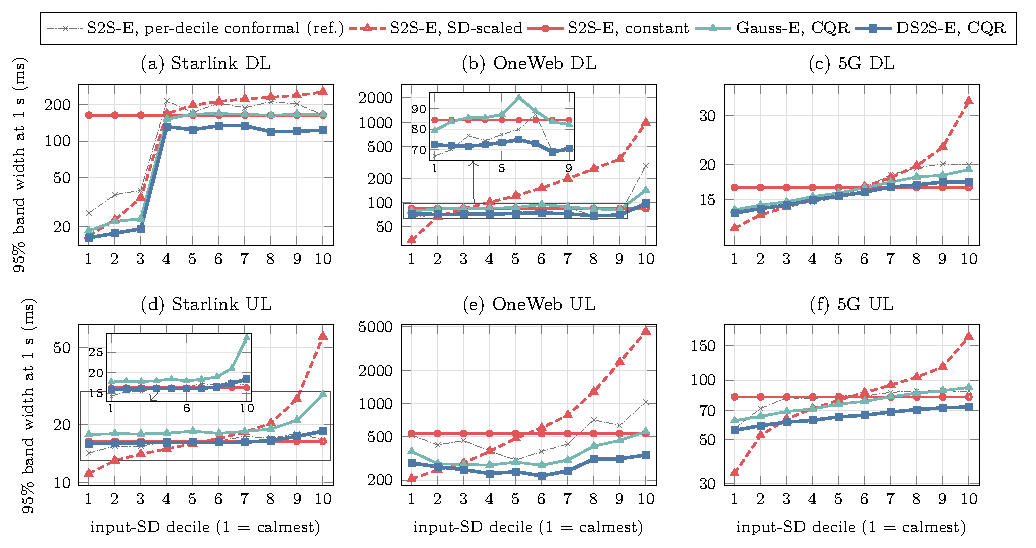
\includegraphics[width=\linewidth]{figs_pdf/fr_condwidth.pdf}
  \caption{Mean width of the calibrated 95\% RTT interval at 1\,s ahead per input-SD decile. The constant interval has one width. DS2S-E adapts its width to the regime: on Starlink DL it is \WidDSSLDLcalmLo{} to \WidDSSLDLcalmHi\,ms in the idle deciles and \WidDSSLDLloadLo{} to \WidDSSLDLloadHi\,ms in the loaded ones, against \WidConstSLDL\,ms for the constant interval. The per-decile conformal interval is a reference that uses the binning variable. Insets: zoom where the curves overlap.}
  \label{fig:condwidth}
\end{figure}

\begin{table}[H]
\centering
\caption{Coverage gap $\max_d|\mathrm{cov}_d-0.95|$ over input-SD deciles and interval score (ms) of all 95\% RTT intervals on the test sessions. SD: scaled by the input SD with a small floor. SD-tuned: floor chosen on the calibration sessions. Per-dec.$^\dagger$: conformal per input-SD decile, a reference that uses the binning variable, not bolded. Bold: best of the other intervals.}
\label{tab:condcovall}
\resizebox{\linewidth}{!}{% generated by modeling/experiments/fr_condcov.py (RTT, 95% bands, TEST windows)
% gap = max over input-SD deciles (edges from validation) of |coverage - 0.95|, coverage pooled over the 15 steps
% SD = band scaled by the input SD (small eps), SD-tuned = eps picked on validation,
% per-dec. = Mondrian conformal per input-SD decile (uses the binning variable, reference only)
\begin{tabular}{lccccccc}
\toprule
 & \multicolumn{4}{c}{S2S-E point forecast + conformal} & \multicolumn{3}{c}{quantile forecast + CQR} \\
\cmidrule(lr){2-5}\cmidrule(lr){6-8}
Link & const. & SD & SD-tuned & per-dec.$^\dagger$ & LQR & Gauss-E & DS2S-E \\
\midrule
\multicolumn{8}{l}{\emph{coverage gap $\max_d|\mathrm{cov}_d-0.95|$}} \\
OneWeb DL & 0.055 & 0.178 & 0.026 & 0.013 & \textbf{0.020} & 0.154 & 0.062 \\
OneWeb UL & 0.056 & 0.106 & \textbf{0.015} & 0.030 & 0.023 & 0.034 & 0.051 \\
Starlink DL & 0.048 & 0.036 & 0.038 & 0.030 & 0.061 & 0.045 & \textbf{0.026} \\
Starlink UL & 0.094 & 0.082 & 0.078 & 0.089 & \textbf{0.031} & 0.034 & 0.070 \\
5G DL & 0.027 & 0.041 & 0.015 & 0.009 & \textbf{0.004} & 0.009 & 0.006 \\
5G UL & 0.014 & 0.054 & 0.008 & 0.015 & 0.013 & 0.004 & \textbf{0.003} \\
\midrule
\multicolumn{8}{l}{\emph{interval score (ms)}} \\
OneWeb DL & 323.4 & 416.5 & 316.5 & 318.4 & 263.7 & 298.6 & \textbf{259.0} \\
OneWeb UL & 1027 & 1821 & 995.7 & 1004 & \textbf{742.1} & 789.1 & 756.9 \\
Starlink DL & 243.5 & 208.0 & 206.4 & 202.6 & 152.3 & 176.5 & \textbf{143.4} \\
Starlink UL & 38.2 & 39.2 & 37.9 & 38.1 & \textbf{33.8} & 36.4 & 34.6 \\
5G DL & 25.2 & 25.9 & 25.0 & 24.9 & 22.4 & 23.5 & \textbf{21.7} \\
5G UL & 127.9 & 135.5 & 127.5 & 127.5 & 93.9 & 121.5 & \textbf{91.7} \\
\bottomrule
\end{tabular}
}
\end{table}

The OneWeb links show the limit of DS2S-E. Its coverage gap there is not smaller than that of the constant interval. DS2S-E widens its interval only \WidRatioOWDL{} times (DL) and \WidRatioOWUL{} times (UL) from the calmest to the most volatile tenth, while the calibrated error grows \ErrRatioOWDL{} and \ErrRatioOWUL{} times, and it covers that tenth only at \CovDSOWDLdTen{} and \CovDSOWULdTen. The input carries the warning, since an SD-scaled interval with a tuned floor covers the same tenth at \CovNormTunedOWDLdTen{} and \CovNormTunedOWULdTen. DS2S-E under-reacts to the rare OneWeb bursts. Fig.~\ref{fig:condwidth} shows the widths behind these numbers.

\subsection{Where the Interval-Score Gain Comes From}
We built intermediate intervals that change one ingredient at a time, all calibrated on the same sessions. Moving a constant interval from the S2S-E mean to the DS2S-E mean changes the score by \DecCentreLo\% to $+$\DecCentreHi\%. The better center is not the source. Giving the S2S-E forecast the per-window width of DS2S-E, placed symmetrically, gains \DecWidthLoAbs\% to \DecWidthHiAbs\%. Placing the interval asymmetrically, as DS2S-E does, gains another \DecAsymLoAbs\% to \DecAsymHiAbs\%. The adaptive width carries most of the gain on Starlink DL and OneWeb UL. The skew carries most of it on 5G UL, where the raw DS2S-E interval at 1\,s reaches \AsymQULratio{} times further above its median than below it.

\subsection{How Specific Is the Gain to the Final Model?}
Table~\ref{tab:extent} lists the interval score and the coverage gap of the intervals that a deployed system could use, all calibrated on the calibration sessions. First, no interval around the S2S-E point forecast comes close to the quantile forecasters. The asymmetric interval helps where the skew is strong and the SD-scaled one where the regime shows in the input SD, but the best of them is still \ExtBestPointLoAbs\% to \ExtBestPointHiAbs\% worse than DS2S-E on every link. Second, the new inputs and the anchored decoder do not explain the gain. S2S-AE-E shares them with DS2S-E but outputs a mean, and it changes the interval score of S2S-E by only \ExtFrfullLo\% to $+$\ExtFrfullHi\%. \GaussSentence{} Fourth, the linear quantile model LQR does almost as well as DS2S-E. It is within \ExtLQRMaxAbs\% of DS2S-E on every link and better on OneWeb UL and Starlink UL, and DS2S-E is significantly better only on \LQRsigLinks, by \LQRsigLo\% to \LQRsigHi\%. The source of the gain is therefore the distributional output calibrated across sessions, which a linear model can exploit too. What the recurrent network adds is a better point forecast: against LQR, DS2S-E lowers the RMSE on all six links (\LQRRMSELoAbs\% to \LQRRMSEHiAbs\%, all significant).

\begin{table}[H]
\centering
\caption{Interval score (IS, ms) and coverage gap over input-SD deciles of the 95\% RTT intervals on the test sessions. SD-scaled: floor tuned on the calibration sessions. S2S-AE-E: the inputs and decoder of DS2S-E with a scalar output. Bold: lowest IS of the link. GS2S-E \GaussSeedNote.}
\label{tab:extent}
\resizebox{\linewidth}{!}{%
\begin{tabular}{ll*{12}{r}}
\toprule
 & & \multicolumn{2}{c}{OneWeb DL} & \multicolumn{2}{c}{OneWeb UL} & \multicolumn{2}{c}{Starlink DL} & \multicolumn{2}{c}{Starlink UL} & \multicolumn{2}{c}{5G DL} & \multicolumn{2}{c}{5G UL} \\
\cmidrule(lr){3-4}\cmidrule(lr){5-6}\cmidrule(lr){7-8}\cmidrule(lr){9-10}\cmidrule(lr){11-12}\cmidrule(lr){13-14}
Forecast & Interval & IS & gap & IS & gap & IS & gap & IS & gap & IS & gap & IS & gap \\
\midrule
\tabinput{data/tab_extent.tex}
\bottomrule
\end{tabular}}
\end{table}
